\documentclass[12pt,a4paper]{article}

\usepackage{fontspec}
\IfFontExistsTF{Times New Roman}
  {\setmainfont{Times New Roman}}
  {\IfFontExistsTF{CMU Serif}
    {\setmainfont{CMU Serif}}
    {\setmainfont{DejaVu Serif}}}
\IfFontExistsTF{Cascadia Mono}
  {\setmonofont{Cascadia Mono}}
  {\IfFontExistsTF{DejaVu Sans Mono}
    {\setmonofont{DejaVu Sans Mono}}
    {\setmonofont{CMU Typewriter Text}}}

\usepackage{geometry}
\geometry{left=25mm,right=15mm,top=20mm,bottom=20mm}
\setlength{\emergencystretch}{3em}
\usepackage{amsmath}
\usepackage{fvextra}
\usepackage{graphicx}
\usepackage{hyperref}
\hypersetup{hidelinks}

\title{Отчёт по задаче <<Китайский почтальон>>}
\author{Смола Артём, группа 23.Б08}
\date{}

\begin{document}
\maketitle

\section{Постановка задачи}
Дан связный неориентированный взвешенный граф.
Требуется найти минимальную длину замкнутого маршрута, который проходит по каждому ребру графа хотя бы один раз.

\section{Принцип решения}
Если все вершины имеют чётную степень, граф эйлеров, и ответ равен сумме длин всех рёбер.
Если есть вершины нечётной степени, часть рёбер нужно пройти повторно.

Алгоритм:
\begin{enumerate}
    \item Посчитать сумму длин всех рёбер.
    \item Найти множество вершин нечётной степени.
    \item Для всех нечётных вершин посчитать попарные кратчайшие расстояния.
    \item Для поиска расстояний использовать алгоритм Дейкстры.
    \item Найти минимальное попаривание нечётных вершин методом динамики по битовой маске.
    \item Ответ:
    \[
    \text{sum\_edges} + \text{min\_matching\_cost}.
    \]
\end{enumerate}
В данной реализации кратчайшие пути ищутся алгоритмом Дейкстры от каждой нечётной вершины.
Это позволяет не считать полную матрицу всех пар вершин, как в алгоритме Флойда,
и обычно даёт лучшую практическую скорость на разреженных графах.

\section{Корректность}
Если все степени вершин чётные, граф эйлеров.
Тогда существует маршрут, проходящий по каждому ребру ровно один раз, а его длина равна сумме рёбер.

Если есть нечётные вершины, в любом эйлеровом дополнении они должны быть разбиты на пары
добавленными проходами по путям.
Минимальная добавка равна стоимости минимального попаривания нечётных вершин по метрике кратчайших путей.

Динамическое программирование по битовой маске перебирает все корректные попаривания и выбирает минимум.
Значит, итог
\[
\text{sum\_edges} + \text{min\_matching\_cost}
\]
оптимален.

\section{Ограничения реализации}
\begin{itemize}
    \item число нечётных вершин ограничено: $k \le 22$;
    \item при $k > 22$ программа завершает работу с ошибкой;
    \item веса рёбер предполагаются неотрицательными.
\end{itemize}

\section{Исходный код}
Исходный код программы и тестовые данные доступны в репозитории GitHub:
\url{https://github.com/artem-smola/formal_lang}.

\section{Код программы}

Код программы:

{\small
\VerbatimInput[
    fontsize=\footnotesize,
    breaklines=true,
    breakanywhere=true
]{../../Code/main.cpp}
}

\section{Демонстрация работы программы}
\subsection*{1) Входные данные}
\textbf{Рассматриваемый тест:} \texttt{test2}.

Формат входных данных:
\begin{enumerate}
    \item $n,\,m$ --- число вершин и число рёбер.
    \item Далее $m$ строк вида $u\ v\ w$, где $u$ и $v$ --- концы ребра, $w \ge 0$ --- вес ребра.
\end{enumerate}
Ограничения: граф неориентированный, а вершины с ненулевой степенью лежат в одной компоненте связности.

{\small
\VerbatimInput[
    fontsize=\footnotesize,
    breaklines=true,
    breakanywhere=true
]{../../Code/tests/test2.in}
}

\subsection*{2) Вывод}

\begin{center}
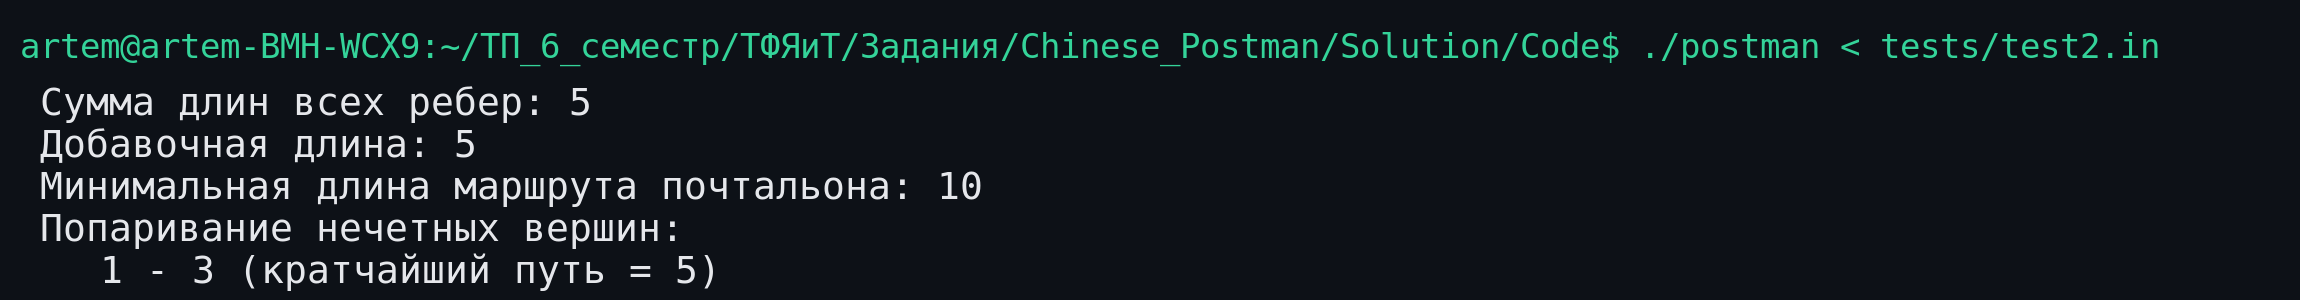
\includegraphics[
    width=\textwidth,
    keepaspectratio
]{assets/terminal_output_test2.png}
\end{center}

\subsection*{3) Визуализация}
\IfFileExists{../../Visualization/test2.png}{
\begin{center}
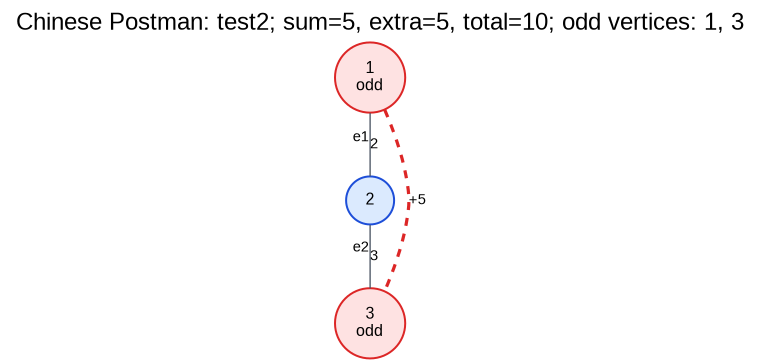
\includegraphics[
    width=\textwidth,
    height=0.38\textheight,
    keepaspectratio
]{../../Visualization/test2.png}
\end{center}
}{
\textbf{Файл визуализации:} \texttt{../../Visualization/test2.dot}

{\small
\VerbatimInput[
    fontsize=\footnotesize,
    breaklines=true,
    breakanywhere=true
]{../../Visualization/test2.dot}
}
}

\subsection*{4) Описание результата}

Для теста \texttt{test2}:
\begin{itemize}
    \item сумма длин всех рёбер равна $5$;
    \item добавочная длина равна $5$;
    \item минимальная длина маршрута почтальона равна $10$;
    \item для нечётных вершин выбрано попаривание $1 \leftrightarrow 3$.
\end{itemize}
Это соответствует классическому решению задачи китайского почтальона: к сумме рёбер добавляется минимальная стоимость попаривания нечётных вершин.

\subsection*{5) Дополнительный граничный тест}
Для \texttt{test1} все степени вершин уже чётные, поэтому:

\textbf{Входные данные теста \texttt{test1}:}

{\small
\VerbatimInput[
    fontsize=\footnotesize,
    breaklines=true,
    breakanywhere=true
]{../../Code/tests/test1.in}
}

\[
\text{добавочная длина} = 0,\qquad
\text{ответ} = \text{сумма рёбер}.
\]
Это проверяет граничный случай эйлерова графа, где дублирование рёбер не требуется.

\section{Анализ сложности}
Пусть:
\begin{itemize}
    \item $n$ --- число вершин;
    \item $m$ --- число рёбер;
    \item $k$ --- число вершин нечётной степени ($k$ всегда чётно).
\end{itemize}

Кратчайшие пути от каждой нечётной вершины:
\[
O(k \cdot m \log n).
\]

Динамика по маске для минимального попаривания:
\[
O(2^k \cdot k^2).
\]

Итоговая сложность:
\[
O(k \cdot m \log n + 2^k \cdot k^2).
\]

Память:
\[
O(n + m + 2^k).
\]

\end{document}
